% Small introduction to tikz figures and its basics, can be found on 
% http://cremeronline.com/LaTeX/minimaltikz.pdf

% Under the file tikz_magic.tex all the different boxes can be found!

\begin{figure}
\begin{tikzpicture}
%Peripheral
\node[fill = {rgb:red,0;green,1;blue,3},box] (Sensor) at (0,0) {Sensor};
\node[fill = {rgb:red,0;green,1;blue,3},box] (RC) at ($(0,-2)+(Sensor)$) {Remote};
%FPGA
\node[fill = black!40!green,box] (Reg) at ($(3.5,0)+(Sensor)$) {Regulator};
\node[fill = black!40!green,box] (Cont) at ($(0,-2)+(Reg)$) {Control};
\node[fill = black!40!green,box] (PWM) at ($(3,0)+(Cont)$) {PWM};
\node[fill = {rgb:red,0;green,1;blue,3},box] (Mot) at ($(3.5,0)+(PWM)$) {Motor \\ Driver};

\draw[->, ultra thick] (RC) -- (Cont);
\draw[->, ultra thick] (Cont) -- (PWM);
\draw[->, ultra thick] (PWM) -- (Mot);
\draw[->, ultra thick] (Sensor) -- (Reg);
\draw[->, ultra thick] (Reg) -- (Cont);

\draw[thick,dashed] ($(-1.5,2)+(Reg)$) -- ($(1.5,4)+(PWM)$) -- ($(1.5,-1.5)+(PWM)$) -- ($(-1.5,-1.5)+(Cont)$) -- ($(-1.5,2)+(Reg)$);
\node[] at ($(1.5,1.5)+(Reg)$) {\textbf{FPGA}};
\end{tikzpicture}%
\caption{simpel Tikz figure}
\end{figure}



%%%%%%%%%%%%%%%%%%%%%%%%%%%%%%%%%%%%%%%%%%%%%%%%%%%%%%%%%%%%%%%%%%%%%%%%%%%%%%%%%%
%%%%%%%%%%%%%%%%%%%%%%%%%%%%%%%%%%%%%%%%%%%%%%%%%%%%%%%%%%%%%%%%%%%%%%%%%%%%%%%%%%


\begin{figure}
\begin{tikzpicture}
%Peripheral
\node[fill = {rgb:red,1;green,2;blue,5},box] (Sensor) at (0,0) {Sensor};
\node[fill = {rgb:red,1;green,2;blue,5},box] (ADC) at ($(0,-2.5)+(Sensor)$) {ADC};
\node[fill = {rgb:red,1;green,2;blue,5},box] (RC) at ($(0,-2.5)+(ADC)$) {Remote};

%FPGA
\node[fill = black!40!green,box] (ADCH) at ($(3.5,0)+(RC)$) {ADC \\ Handler};
\node[fill = black!40!green,box] (DeB) at ($(0,-2.5)+(ADCH)$) {Debouncing};
\node[fill = black!40!green,box] (Convrc) at ($(3.5,0)+(ADC)$) {RC \\ Conversion};
\node[fill = black!40!green,box] (Convs) at ($(3.5,2.5)+(ADC)$) {Sensor \\ Conversion};
\node[fill = black!40!green,box] (Reg) at ($(3,0)+(Convs)$) {Regulator};
\node[fill = black!40!green,box] (Cont) at ($(3,0)+(Convrc)$) {Control};
\node[fill = black!40!green,box] (PWM) at ($(3,0)+(Cont)$) {PWM};
\node[fill = {rgb:red,1;green,2;blue,5},box] (Mot) at ($(3,0)+(PWM)$) {Motor \\ Driver};

\draw[->, ultra thick] ([yshift=-0.4cm]RC) -| ++(1.5,0) |- (DeB);
\draw[->, ultra thick] (RC) -- (ADC);
\draw[->, ultra thick] (DeB) -| (Cont);
\draw[->, ultra thick] (Cont) -- (PWM);
\draw[->, ultra thick] (PWM) -- (Mot);
\draw[->, ultra thick] (Sensor) -- (ADC);
\draw[->, ultra thick] ([yshift=0.6cm]ADC) -| ++(1.5,0) |- (Convs);
\draw[->, ultra thick] (ADC) -- (Convrc);
\draw[<-, ultra thick] ([yshift=-0.4cm]ADC.east) -| ++(0.5,0) |- ([yshift=0.4cm]ADCH);
\draw[->, ultra thick] (Convs) -- (Reg);
\draw[->, ultra thick] (Reg) -- (Cont);
\draw[->, ultra thick] (Convrc) -- (Cont);

\draw[thick,dashed] ($(-1.5,2)+(Convs)$) -- ($(1.5,4.5)+(PWM)$) -- ($(1.5,-6.5)+(PWM)$) -- ($(-1.5,-1.5)+(DeB)$) -- ($(-1.5,2)+(Convs)$);
\node[] at ($(0,1.5)+(Reg)$) {\textbf{FPGA}};
\end{tikzpicture}%
\caption{Advance Tikz figure to shift line position}
\end{figure}


%%%%%%%%%%%%%%%%%%%%%%%%%%%%%%%%%%%%%%%%%%%%%%%%%%%%%%%%%%%%%%%%%%%%%%%%%%%%%%%%%%
%%%%%%%%%%%%%%%%%%%%%%%%%%%%%%%%%%%%%%%%%%%%%%%%%%%%%%%%%%%%%%%%%%%%%%%%%%%%%%%%%%

\begin{figure}
\begin{tikzpicture}

\node[box] (Initialization) at (0,0) {Initialization};
\node[box] (Receive) at ($(0,-2)+(Initialization)$) {Read the data \\if some were received};
\node[box] (Send) at ($(0,-2)+(Receive)$) {Send if the\\ control changed};
\node[box] (Sleep) at ($(0,-2)+(Send)$) {Sleep};
\node[box] (Update_State) at ($(5,0)+(Receive)$) {Update the data\\ available for higher\\level processes};

\draw[->, ultra thick] (Initialization) -- (Receive);
\draw[->, ultra thick] (Receive) -- (Update_State);
\draw[->, ultra thick] (Receive) -- (Send);
\draw[->, ultra thick] (Send) -- (Sleep);
\draw[->, ultra thick] (Sleep.west) -| ++(-2,0) |- (Receive);

\end{tikzpicture}
\caption{Before}
\end{figure}

%%%%%%%%%%%%%%%%%%%%%%%%%%%%%%%%%%%%%%%%%%%%%%%%%%%%%%%%%%%%%%%%%%%%%%%%%%%%%%%%%%
%%%%%%%%%%%%%%%%%%%%%%%%%%%%%%%%%%%%%%%%%%%%%%%%%%%%%%%%%%%%%%%%%%%%%%%%%%%%%%%%%%

\begin{figure}
\begin{tikzpicture}

\node[box] (Initialization) at (0,0) {Initialization};
\node[box] (Receive) at ($(6,-3)+(Initialization)$) {Asynchronous reading};
\node[box] (Update_State) at ($(0,-2)+(Receive)$) {Process the data\\and update them for\\ higher level processes};
\node[box] (Send) at ($(0,-3)+(Initialization)$) {Send if the\\ control changed};
\node[box] (Sleep) at ($(0,-2)+(Send)$) {Sleep};


\draw[->, ultra thick] (Initialization.south) -- ++(0,-0.5) -|  (Receive.north);
\draw[->, ultra thick] (Initialization) -- (Send);
\draw[->, ultra thick] (Receive) -- (Update_State);
\draw[->, ultra thick] (Update_State.west) -| ++(-1,0) |- (Receive);
\draw[->, ultra thick] (Send) -- (Sleep);
\draw[->, ultra thick] (Sleep.west) -| ++(-1,0) |- (Send);


\end{tikzpicture}
\caption{After}
\end{figure}


%%%%%%%%%%%%%%%%%%%%%%%%%%%%%%%%%%%%%%%%%%%%%%%%%%%%%%%%%%%%%%%%%%%%%%%%%%%%%%%%%%
%%%%%%%%%%%%%%%%%%%%%%%%%%%%%%%%%%%%%%%%%%%%%%%%%%%%%%%%%%%%%%%%%%%%%%%%%%%%%%%%%%

\begin{figure}
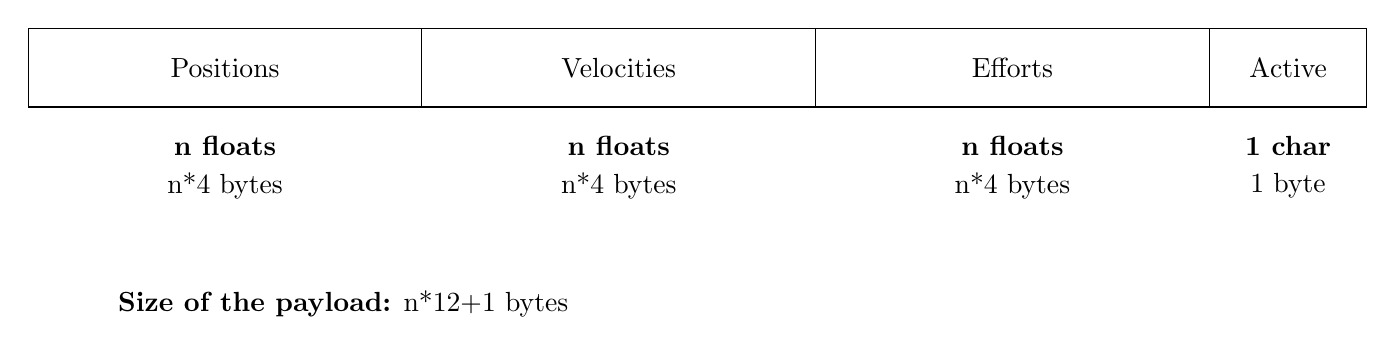
\begin{tikzpicture}

\draw (0,0) rectangle (17,1);
\draw (0,0) rectangle (5,1);
\draw (0,0) rectangle (10,1);
\draw (0,0) rectangle (15,1);

\node at (2.5,0.5) {Positions};
\node at (7.5,0.5) {Velocities};
\node at (12.5,0.5) {Efforts};
\node at (16,0.5) {Active};

\node at (2.5,-0.5) {\textbf{n floats}};
\node at (7.5,-0.5) {\textbf{n floats}};
\node at (12.5,-0.5) {\textbf{n floats}};
\node at (16,-0.5) {\textbf{1 char}};

\node at (2.5,-1) {n*4 bytes};
\node at (7.5,-1) {n*4 bytes};
\node at (12.5,-1) {n*4 bytes};
\node at (16,-1) {1 byte};

\node at (4,-2.5) {\textbf{Size of the payload:} n*12+1 bytes}; %I have no idea why i need to put 4 as a coordinate for it to not mess up the rest of the figure
\end{tikzpicture}
\caption{Received packet for n motors}
\end{figure}

%%%%%%%%%%%%%%%%%%%%%%%%%%%%%%%%%%%%%%%%%%%%%%%%%%%%%%%%%%%%%%%%%%%%%%%%%%%%%%%%%%
%%%%%%%%%%%%%%%%%%%%%%%%%%%%%%%%%%%%%%%%%%%%%%%%%%%%%%%%%%%%%%%%%%%%%%%%%%%%%%%%%%

\begin{figure}
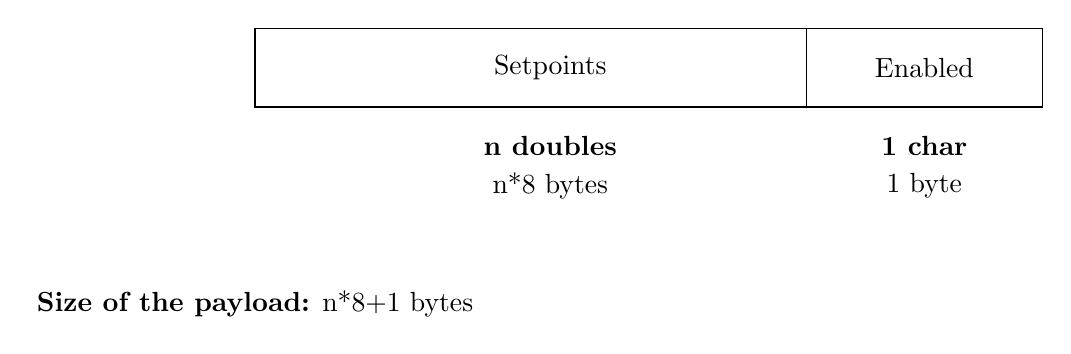
\begin{tikzpicture}

\draw (0,0) rectangle (10,1);
\draw (0,0) rectangle (7,1);

\node at (3.75,0.5) {Setpoints};
\node at (8.5,0.5) {Enabled};

\node at (3.75,-0.5) {\textbf{n doubles}};
\node at (8.5,-0.5) {\textbf{1 char}};

\node at (3.75,-1) {n*8 bytes};
\node at (8.5,-1) {1 byte};

\node at (0,-2.5) {\textbf{Size of the payload:} n*8+1 bytes}; 
\end{tikzpicture}
\caption{Sent packet for n motors}
\end{figure}